% From AAAI 2018 template
\def\year{2018}\relax
%File: formatting-instruction.tex
\documentclass[letterpaper]{article} %DO NOT CHANGE THIS
\usepackage{aaai18}  %Required
\usepackage{times}  %Required
\usepackage{helvet}  %Required
\usepackage{courier}  %Required
\usepackage{url}  %Required
\usepackage{graphicx}  %Required
\frenchspacing  %Required
\setlength{\pdfpagewidth}{8.5in}  %Required
\setlength{\pdfpageheight}{11in}  %Required
\setcounter{secnumdepth}{2}  

\graphicspath{ {images/} }
\usepackage{amsfonts}
\usepackage{amsmath}
\usepackage{comment}
\usepackage{float}
\usepackage{import}
\usepackage{multirow}
\usepackage{subfigure}
\usepackage{tikz}
\usetikzlibrary{positioning}
\usepackage[inline]{enumitem}
\usepackage{amsthm}

\usepackage{soul}

% Configuration
%\DeclareMathSizes{ds}{ts}{ss}{sss}
\DeclareMathSizes{10}{9}{7}{5}   % For size 10 text
%\DeclareMathSizes{11}{19}{13}{9}   % For size 11 text
%\DeclareMathSizes{12}{20}{14}{10}  % For size 12 text

%%%%%%%%% Macros %%%%%%%%%%%%%%%%%%
\newtheorem{defn}{Definition}
\newif\ifblind
\def\goldenr{1.618}
\newcommand*\textfrac[2]{
      \frac{\text{#1}}{\text{#2}}
  }
\newcommand{\TODO}[1]{TODO:{#1}}
\newcommand{\etal}{et~al.}
\def\state{s}
\def\statet{\state_t}
\def\statetp{\state_{t-1}}
\def\statetn{\state_{t+1}}
\def\obs{o}
\def\obst{\obs_t}
\def\act{a}
\def\actt{\act_t}
\def\acttp{\act_{t-1}}
\def\acttn{\act_{t+1}}
\def\Obs{\mathcal{O}}
\def\ObsFunc{C}
\def\ObsFuncFull{\ObsFunc(\statet, \actt) \rightarrow \obst}
\def\ObsFuncInv{\ObsFunc^{-1}}
\def\ObsFuncInvFull{\ObsFuncInv(\obst, \statetp, \actt) \rightarrow \statet}
\def\State{\mathcal{S}}
\def\Action{\mathcal{A}}
\def\Trans{T}
\def\TransFull{\Trans(\statet, \actt) \rightarrow \statetn}
\def\TransObs{T_c}
\def\Rew{R}
\def\rew{r}
\def\rewt{\rew_t}
\def\rewtp{\rew_{t-1}}
\def\rewtn{\rew_{t+1}}
\def\RewFull{\Rew(\statet, \actt) \rightarrow \rewtn}
\def\TransObsFull{\TransObs(\statet, \obst, \actt, \rewt; \theta_T) \rightarrow \statetn}
\def\Value{V}
\def\pit{\pi_t}
\def\piDef{\pi(\acttn|\statet, \obst, \actt, \rewt; \theta_\pi) \rightarrow \pit(\acttn ; \theta_\pi)}
\def\Valuet{\Value_t}
\def\ValueDef{\Value(\statet, \obst, \actt, \rewt; \theta_\Value) \rightarrow \Valuet(\theta_\Value)}
\def\R{\mathbb{R}}
\def\E{\mathbb{E}}

%%%%%% Possible titles %%%%%%%%%
% TODO: Finalize title
%\title{Learning to Navigate in Simple Environments}
%\title{What kind of maps to DRL agents remember?}
%\title{How detailed mapping is necessary for navigation?}
%\title{Walking mazes while blinding}
%\title{Robots also text while driving}
%\title{Training robots to text while driving}
%\title{BLINC: Blindfolded curriculumn learning for querying maps from DRL agents}
%\title{Learning to navigate or learning to repeat?}
%\title{Do deep reinforcement learning algorithms learn to plan?}
\title{Deep Reinforcment Learning and the Navigation Myth}

\blindtrue
\ifblind
\author{Authors omitted for blind review}
\else
\author{Shurjo Banerjee\thanks{indicates equal contribution}
  \and Vikas Dhiman\footnotemark[1]
  \and Brent Griffin
  \and Jason J. Corso\\
  \texttt{\{shurjo,dhiman,griffb,jjcorso\}@umich.edu}
\\Electrical Engineering and Computer Science Department
\\University of Michigan, Ann Arbor, USA
}
\fi


\makeatletter
% Update PDF meta data
\pdfinfo{
/Title (\@title)
/Author (See paper)}
\makeatother

\begin{document}
\maketitle
\begin{abstract}

Deep reinforcement learning (DRL) algorithms have demonstrated strong progress in learning to reach a goal in challenging environments.  One might conclude that state of the art DRL agents, such as \cite{MiPaViICLR2017}, learn to navigate by learning a some form of a map followed by path planning to goal.  Yet, from this earlier work, it is not clear whether or not these DRL agents are indeed doing any form of path planning.  In this paper, we pose and study this question: are DRL agents doing some form of path-planning?  Our experiments show that the agents are not memorizing the maps of mazes at the training stage but, rather, memorizing the maps of mazes at the testing stage, for each maze differently.  However, the DRL agents fall short of qualifying as mapping and path-planning agents.  We find evidence that the DRL agents are learning a correspondence to perform an action for each frame and there is no evidence of path-planning.

\end{abstract}
\section{Introduction}
%\input{intro-drl-is-hot}
%\input{intro-drl-and-mapping}
%% Outline
% 1. Navigation is important problem
% 1.5 Traditionally addressed by mapping during exploration and path
%      planning during exploitation.
% 2. End to end learning algorithms have shown promise to take over
%      mapping and path
% 3. We do not know how these algorithms work. There has been work in computer vision that shows the learning on neural network based methods can be learning totally different kind of patterns from what we would expect.
% 4.1 We find that it is not remembering the map it is being trained on
% 4.2 We find that no path planning is  happening only, memorizing and regeneration of the sequence of steps. However, it is not 

% 1. Navigation is important problem
% 1.5 Traditionally addressed by mapping during exploration and path
%      planning during exploitation.
Navigation remains a fundamental problems in mobile robotics and artificial intelligence~\cite{SmChIJRR1986,ElCOMPUTER1980}.
The problem is classically addressed by separating the eventual task of navigation into exploration and exploitation. 
In exploration the environment is represented in some sort of \emph{map} data-structure. 
In exploitation, the map is used for localization and path-planning to find a path to a desired destination based on given optimality criterion. 
This classical approach, traditionally called SLAM (Simulataneous Localization and Mapping), constitutes an entire subfield of robotics whose successes include the birthing of the autonomous driving industry. 
SLAM however, possesses its own limitations. Algorithms, especially those centered in vision, lack performance invariance often failing to extend results to environments that are subtly different from the ones they were trained on. As a simple example, state-of-the-art monucular SLAM methods fail when confronted with textureless environments.

More recently, end-to-end navigation methods---methods that attempt to  
solve the navigation problem without breaking it down into separate parts of localization, mapping and path-planning---have gained traction.
%
% 2. End to end learning algorithms have shown promise to take over
%      mapping and path-planning
With the recent advances of Deep Reinforcement Learning (DRL) \cite{MnKaSiNATURE2015}, these end-to-end navigation methods \cite{MnBaMiICML2016,SiHuMaNATURE2016,LePaKrISER2017,MiPaViICLR2017,OhChSiICML2016} forego decisions about the details that are required in the intermediate step of mapping.
The potential for simpler yet capable methods is rich; for example, one can optimize to store only the minimal amount of map information that is required perform the end objective of a navigation task.
One such work, \cite{MiPaViICLR2017}, has demonstrated advances in this task of navigation creating agents that are able to explore and find goals in complicated, three-dimensional worlds without the provision of any externally-supplied map like concept or memory strcutures. 

using only the first-person monocular view in randomly generated mazes. Not only their algorithm shows evidence of localization, but they also show some of evidence of better than random path planning when the goal location is randomly chosen during evaluation time. 
:q

\begin{figure}
%\rotatebox{90}{\hspace{3em}Trained on 1 map }
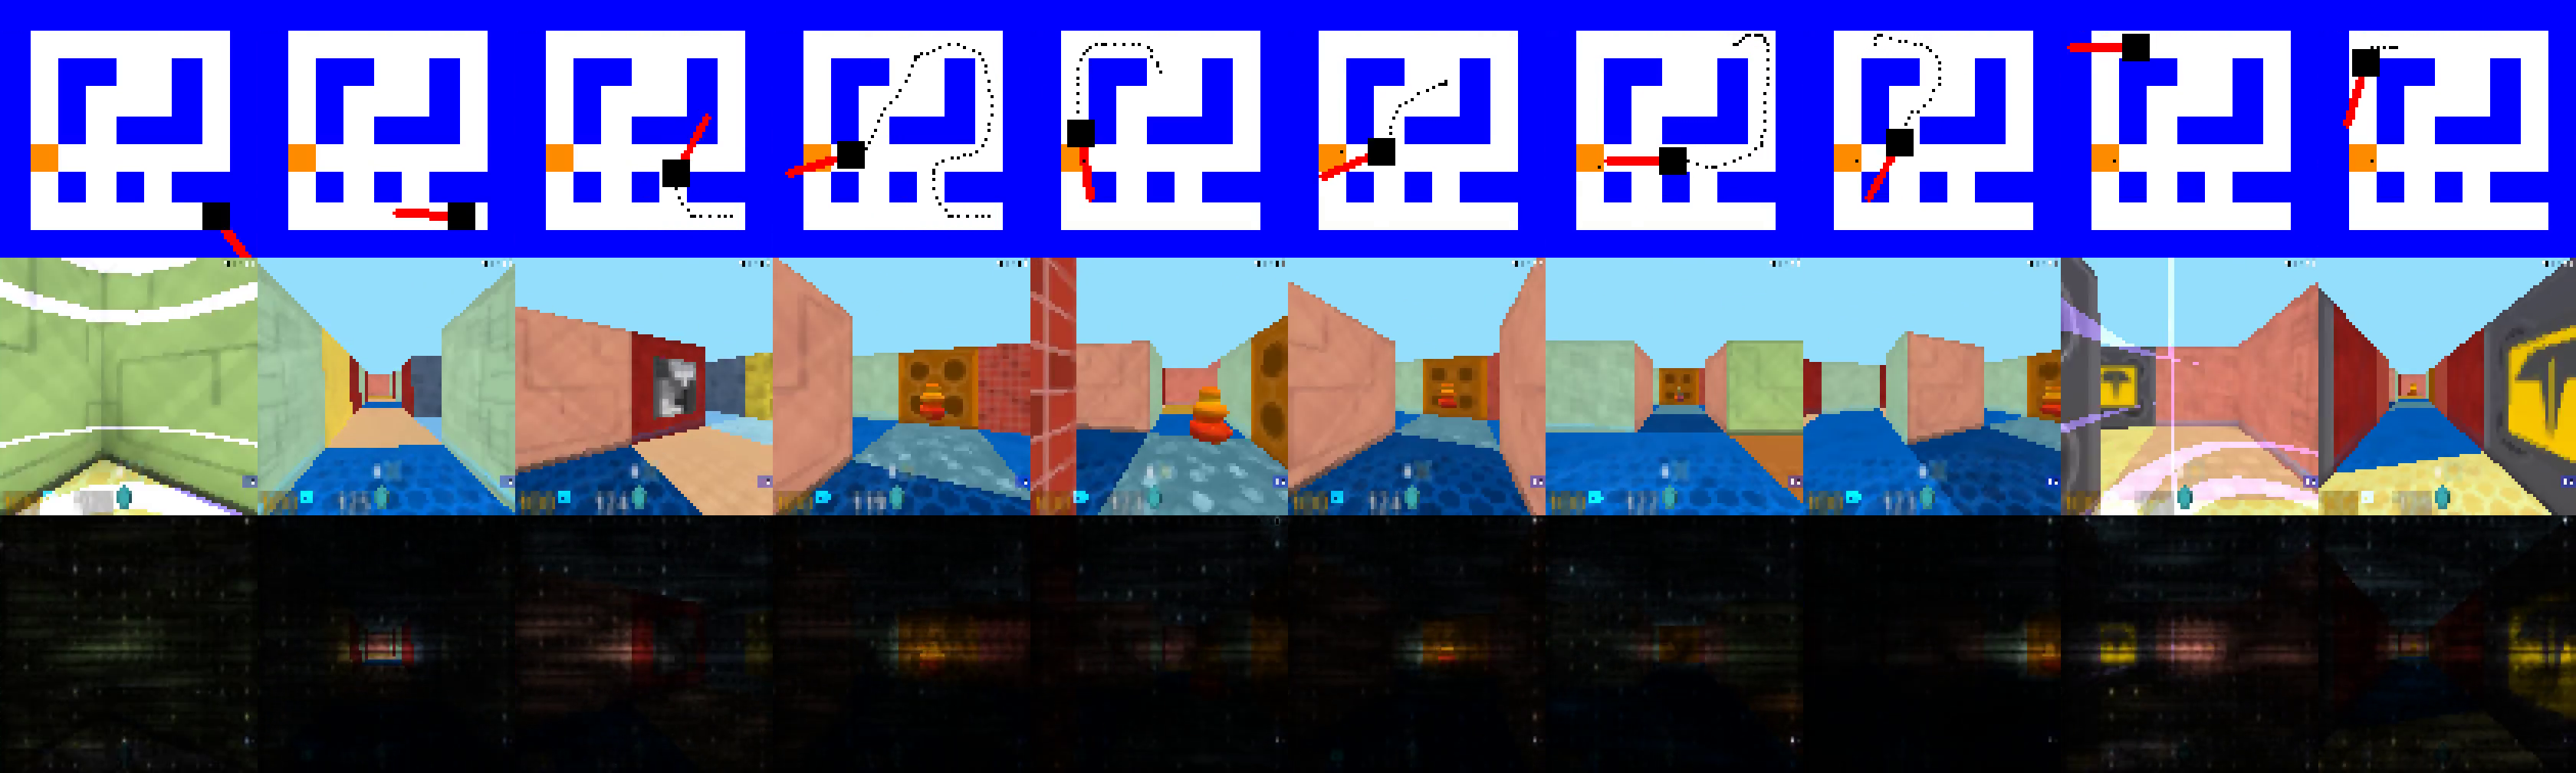
\includegraphics[width=\textwidth]{./exp-results/training-09x09-0127-on-0127.png}
%\rotatebox{90}{\hspace{2em}Trained on 1000 maps }
%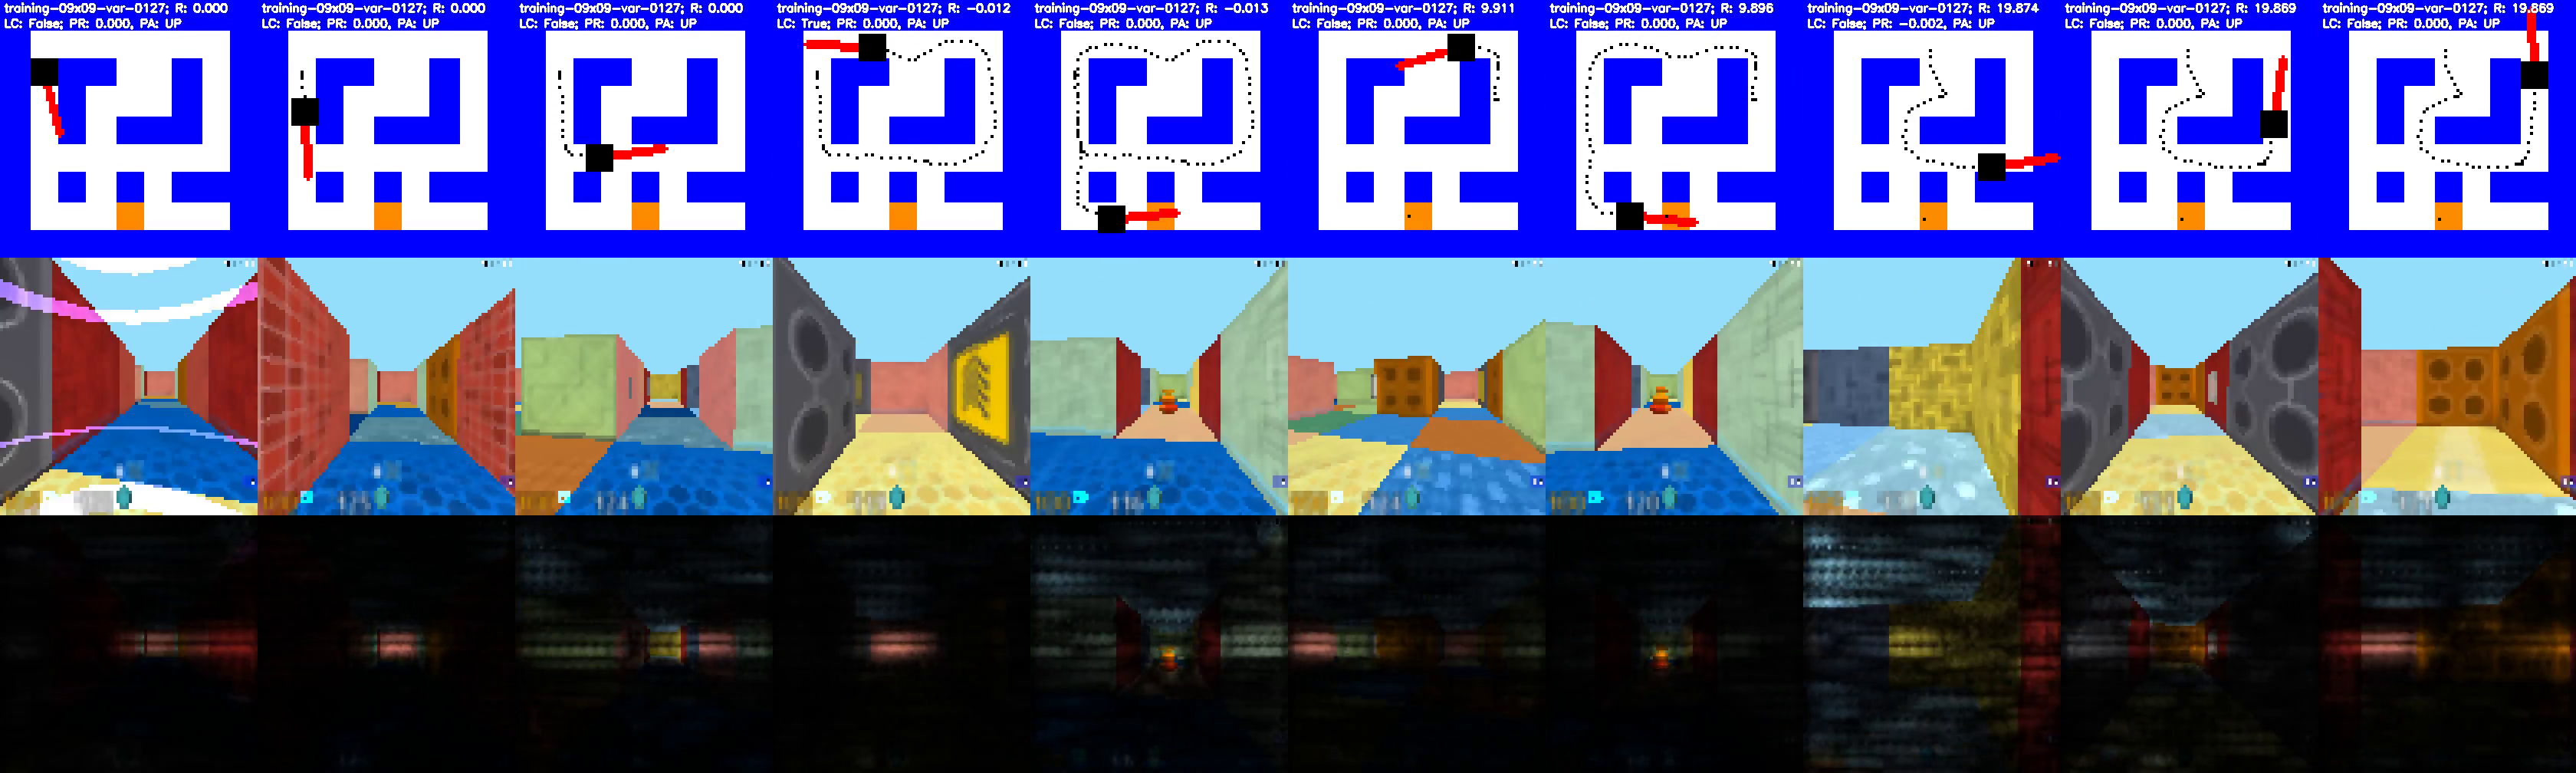
\includegraphics[width=\textwidth]{./exp-results/training-1000-on-0127.png}
\caption{Qualitative results of evaluating algorithm on map id 127. The top three rows show selected frames for the algorithm trained on the same map 127, while the bottom three rows show the result of evaluting the algorithm trained on 1000 maps evaluated on 127. The top row shows the top view of the robot moving through the maze, second row shows the first person which is the only input available to the agent (except reward). The third row shows the attention masked view of the algorithm. We observe that the algorithm focuses attention at the horizon in long corridors, on the goal object (it looks like stacked rings) and on interesting decals.}
\label{fig:training-qualitative}
\end{figure}

% 3. We do not know how these algorithms work. There has been work in computer vision that shows the learning on neural network based methods can be learning totally different kind of patterns from what we would expect.
Despite this potential and recent successes, 
state-of-the-art DRL based methods have been confronted with their own set of problems, such as difficulty to understand the method limitations or the kind of patterns the algorithm is understanding.  The black-box nature of these methods make them hard to study.
On similar lines, \cite{NgYoClCVPR2015} show that neural-network-based object detection methods can be easily fooled by introducing noise that is imperceptible to humans. Hence, it is important to analyze the DRL methods to understand if they are truly ``learning to navigate'' \cite{MiPaViICLR2017}.

% 4.1 We find that it is not remembering the map it is being trained on
% 4.2 We find that no path planning is  happening only, memorizing and regeneration of the sequence of steps. However, it is not 

In this work, we focus on the work of \cite{MiPaViICLR2017} and analyze the method using multiple random maps with different degrees of randomness. As a generalization, we propose a 4-stage benchmark for end-to-end navigation methods.
Our experimental setup is similar to \cite{MiPaViICLR2017} and uses the same open source library Deepmind's Lab \cite{BeLeTeARXIV2016}.
We setup a maze where the goal is randomly placed and the agent is randomly spawned.
The objective of the agent is to hit the goal as many times as possible within a fixed episode time.
Every time the agent hits the goal, it respawns at a random location.
With this setup \cite{MiPaViICLR2017} found that the agent finds the goal faster the second time onwards as compared to the first time.
This implies that agent is somehow able to exploit the new information about position of the goal to reach the goal faster.
However, \cite{MiPaViICLR2017} do not rule out random chance because they only show the successful result on random goal case with only one map, do not report standard deviation on their metrics and do not evaluate the algorithm on unseen maps.
Even though separting training and testing sets is the obvious thing to do in machine learning, we are the first work to evaluate any DRL based navigation method on unseen maps.
We expand on their analysis and evaluate the same metric on multiple types of maps including randomly generated maps.

We find no evidence of DRL agents being able to perform shortest path-planning in unseen mazes even in simple mazes.
We observe that the agent prefers to take a particular path just as an artifact of initialization.
We hypothesize that the agents are learning a correspondence between local sequence of frames and actions.
These findings are the results on testing and training on multiple maps that were randomly chosen from set of 1100 randomly generated maps.
We provide thorough and clear summary data to substantiate these findings as well as individual maps and results to explain them carefully.
A secondary finding is that even if the agent is trained on a single maze it is able to navigate better than random in unseen mazes.


 
\section{Related Work}
%\input{related-work-papers}
\input{related-work-topical}

\section{Background}
%\subsection{Reinforcement Learning}
\label{sec:background}
Our experimental setup is inspired by Mirowski \etal{} work \cite{MiPaViICLR2017}. We summarize the technical setup here for completeness. We recommend \cite{MnBaMiICML2016,MnBaMiICML2016,MiPaViICLR2017}

The problem of navigation is formulated as interaction between environment and agent. At time time $t$ the agent takes an action $\actt \in \Action$ and observes observation $\obst \in \Obs$ along with a real reward $\rewt \in \R$.
We assume the environment to be Partially Observable Markov Decision Process (POMDP).
In a POMDP the state of the environment $\statet \in \State$ is assumed to be the only information that is propagated over time and both $\obst$ and $\rewt$ are assumed to be independent of previous states given current state and last action. Formally, a POMDP is a six tuple $(\Obs, \ObsFunc, \State, \Action, \Trans, \Rew)$ that is observation space $\Obs$, observation function $\ObsFuncFull$, state space $\State$, action space $\Action$, transition function $\TransFull$ and reward function $\RewFull$ respectively.
For our problem setup, the observation space $\Obs$ is the space of encoded feature vector that can be generated from input image or combination of other inputs, action space $\Action$ contains four actions: rotate left, rotate right, moved forward and move backward and reward function $\Rew$ is defined for each experiment so that the reaching the goal leads to high reward with auxilary reward to encourage certain kind of behavior.

For Deep reinforement learning the state space $\State$ is not hand tuned, instead it is modeled as semantically meaningless \emph{hidden state} of a fixed size float vector.
Also, instead of modeling observation function $\ObsFuncFull$ and $\TransFull$, a combined transition function $\TransObsFull$ is modeled such that it estimates next state $\statetn$ directly considering previous observation as well as reward into account. For policy-based DRL a policy function $\piDef$ and a value function $\ValueDef$ are also modeled. All three functions $\TransObs$, $\pit$, $\Valuet$ share most of the parameters in a way such that $\theta_T \subseteq \theta_{\pi} \cap \theta_\Value$

%Since we aim to estimate $\ObsFuncInv$ and $\Trans$ from experience, we formulate the experience as observation tuples divided into episodes of fixed length $E$.
%Each episode experience contains $E$ tuples with observation, action and corresponding reward $D_E = \{(\obs_0, \act_0, r_0), \dots, (\obs_E, \act_E, r_E)\}$. After each episode the state $\state_t$ is reset to all zeros and another data sequence is collected. Let the collected dataset be $D_N = \{
Our objective is to estimate unknown weights $\theta = \theta_T \cup \theta_\pi \cup \theta_V$ that maximizes the expected future reward, $R_t = \sum_{k=t}^{t_{end} - t} \gamma^{k-t} r_k$, where $\gamma$ is the discount factor,
%
\begin{align}
\theta^* = \arg\max_{\theta} \E[R_t] \,.
\end{align}
%
% need \graphicspath{{images/}}
\def\svgwidth{0.5\columnwidth}%
\begin{figure}%
\input{images/a3c-as-pomdp.pdf_tex}%
\def\svgwidth{0.5\columnwidth}%
\input{images/a3c-as-nn.pdf_tex}
\caption{POMDP on the left, neural network implementation on the right.}
\end{figure}

\paragraph{Asynchronous Advantage Actor-Critic}
\def\charelig{\nabla_{\theta_\pi}\ln \pit(\acttn; \theta_\pi)}
% There are many different variations of RL. There are many different RL algorithms: value-based methods like Q-learning and SARSA and policy-based method like actor-critic.
In this paper we use policy-based method called Asynchronous Advantage Actor-Critic (A3C) \cite{MnBaMiICML2016} that allows weight updates to happen asynchronously in a multi-threaded environment.
It works by keeping a ``shared and slowly changing copy of target network'' that is updated every few iterations by accumulated gradients in each of the threads.
The gradients are never applied to the local copy of the weights, but the local copy of weights is periodically synced from the shared copy of target weights.
The gradient for weight update is proportional to the product of \emph{advantage}, $R_t - \Value_t(\theta_\Value)$, and \emph{characteristic eligibility}, $\charelig$ \cite{WiML1992}, updating the weights according to the following update equations
\begin{align}
  \theta_\pi &\leftarrow \theta_\pi
  + \sum_{t \in \text{episode}}\alpha_\pi \charelig (R_t - \Value_t(\theta_\Value))
  \\
  \theta_\Value &\leftarrow \theta_\Value
  + \sum_{t \in \text{episode}} \alpha_\Value \frac{\partial (R_t - \Value_t(\theta_\Value))^2}
                  {\partial\theta_\Value}
                  \, .
\end{align}

For more details of the A3C algorithm please refer to \cite{MnBaMiICML2016}.

%An agent interacts within an environment, $\varepsilon$. At timestep $t$, the agent observes the current environment state, $s_{t-1}$ and performs an action $a_t$ from the set of allowed actions, $A$. The environment, under the effect of the action, returns then next state $s_t$ and the corresponding reward, $r_t$ upon which the process continues. An agent interacts with the environment over a fixed number of timesteps, called an $episode$. 


%\section{Approach}
%We begin by asking for a definition of map. When can we say that an agent has 
%some notion of map.
%\begin{defn}[Map]
%  A Map is any saved information that enables better than random path planning to a predestined goal which is not within immediate view.
%\end{defn}

\paragraph{Nav A3C}
%In line with \cite{MiPaViICLR2017}, the combined transition function is modeled as two LSTMs (Long Short Term Memory)~\cite{HoScNC1997} stacked over one another.
% Outline
% 1. Describe simulators
% 2. Episode setup
% 3. architecture
% 4. Training
We base our experimental setup on the work of \cite{MiPaViICLR2017} and chose the architecture labeled a modified version of Nav-A3C D\textsubscript{1}D\textsubscript{2}L as shown in Fig.~\ref{fig:nav-a3c}.
Nav-A3C architecture consists of an observation encoder, which can be a Convlutional Neural Network (CNN) for images or a Fully Connected (FC) network for a simpler environment like gridworld, and a recurrent network unit that acts as transition function for each step and its hidden state serving as state space.
Note that reward $\rewt$ and previous action $\act$ to the two LSTMs at different stages.
%
\begin{figure}%
\usetikzlibrary{positioning}
\begin{tikzpicture}
\node[networknode,fill=green!20] at (10.5, 2.5) (lstm2) {LSTM:64};
\node[networknode,fill=green!20,left=0.6 of lstm2] (lstm) {LSTM:256};
\node[networknode,fill=orange!20,left=0.8 of lstm]  (enc2) {\parbox{8ex}{CNN:32\\4x4/2x2}};
\node[networknode,,fill=orange!20,left=0.4 of enc2]  (enc) {\parbox{8ex}{CNN:16\\8x8/4x4}};
\node[left=0.4 of enc, inputvar] (It) {$I_t$:84x84x3};
\node[above=0.1 of It,inputvar] (at) {$\acttp$};
\node[below=0.1 of It,inputvar]  (rt) {$\rewtp$};
\node [right=0.8 of lstm2,outvar] (V)  {$V$, $\pi$};
\node [shift={(-0.4,0)},above=0.4 of V,auxvar] (pi)  {$L$};
\node [shift={(-0.4,0)},below=0.4 of V,auxvar] (D)  {$D_2$};
\draw [-stealth] (It) edge (enc);
\draw [-stealth] (at) edge [in=110,looseness=0.4] (lstm2);
\draw [-stealth] (enc2) edge [bend left=70,looseness=0.4] (lstm2);
\draw [-stealth] (enc) edge (enc2);
\draw [-stealth] (enc2) edge node [shift={(0.225,0.1)},left]{$o_t$} (lstm);
\draw [-stealth] (rt) edge  [bend right,looseness=0.3] (lstm);
\draw [-stealth] (lstm) edge node[below=0.4,auxvar] (D1) {$D_1$} (lstm2);
\draw [-stealth] (lstm) edge [bend left] (D1);
\draw [-stealth] (lstm2) edge [bend right] (pi);
\draw [-stealth] (lstm2) edge  (V);
\draw [-stealth] (lstm2) edge [bend left] (D);
%\draw [use as bounding box] (5.0,1.5) rectangle (12.0, 4.0);
\end{tikzpicture}
\vline%
\begin{tikzpicture}
%\draw [use as bounding box] (0,0) rectangle (1.8in, 3in);
\node[] at (2.3, 2) (It) {$I_t$: 84x84x3};
\node[networknode, above=1.2 of It, text width=45, align=center] (c1) {conv\\
  3x3/2x2,32};
\node[above=1.2 of c1] (ft) {$o_t$: 256};
\draw [-stealth] (c1) edge [out=30, in=-30,looseness=2] node [right] {4x}(c1);
\draw [-stealth] (It) -- (c1);
\draw [-stealth] (c1) -- (ft);
\end{tikzpicture}
\vline%
\begin{tikzpicture}
%\draw [use as bounding box] (0,0) rectangle (1.8in, 3in);
\node[] at (2.3, 2) (It) {$I_t$: 84x84x3};
\node[networknode, above=1.2 of It] (fc) {FC(256)};
\node[above=1.2 of fc] (ft) {$o_t$: 256};
\draw [-stealth] (It) -- (fc);
\draw [-stealth] (fc) -- (ft);
\end{tikzpicture}
%
\caption{Nav A3C architecture on left and two possible Encoders: CNN encoder on center, FC encoder on right. We use CNN encoder for the 3D world while FC encoder for the gridworld.}%
\label{fig:nav-a3c}
\end{figure}
%
We perform experiments on two kind of environments, Gridworld-2D and full Deepmind's Lab 3D environment \cite{BeLeTeARXIV2016}, henceforth called \emph{3D world}. We note that \cite{MiPaViICLR2017} do not evaluate their trained agents on unseen mazes.

To analyze agents ability to construct map while exploration we test the the algorithm we train the agent on 1000 randomly generated maps and test it on 100 randomly generated map. Fig.~\ref{fig:random-mazes} shows some of the randomly generated maps.
\begin{figure}%
\tikz{\draw (0,0) rectangle  node  {Samples of Random mazes generated} (\columnwidth, \columnwidth/\goldenr);}%
\caption{Samples of Random mazes generated}%
\label{fig:random-mazes}%
\end{figure}

%\subsection{Training Paradigm}
\paragraph{Episode setup}
    During each episode, the agent and the goal are randomly initialized within a randomly chosen maze. Apples, with reward +1, are also randomly placed around the maze to encourage exploration. During the course of an episode, if an agent finds the goal it gets reward +10 and it is re-instantiated at a random location within the same maze with same goal location.
%The apples are not re-instantiated once hit.
    During the course of our experiments, agents are trained on subsets of the total number of training maps and validated on all the testing maps. During test time, apples are removed so as to remove "distractions" from the objective of goal finding.

\subsection{Evaluation on unseen environments}
Agents are trained on subsets of the training maps and tested on the training maps. Following are the reward curves for training and testing across the different environments. 

\begin{figure}
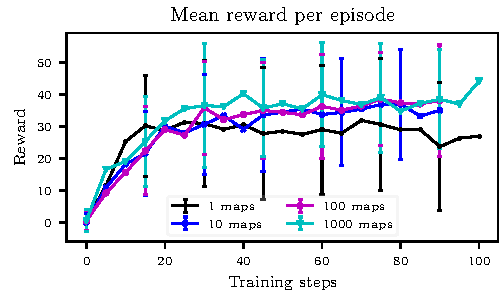
\includegraphics[width=\columnwidth]{images/plot_reward_3D-1000.pdf}
\caption{Mean reward while tested on 100 unseen maps, while being trained on different number of training maps. Note that while training on 1000 maps eventually achieves high reward, it is only higher mean reward (44.2), training on 1 map hits the maximum (31) much faster.}
\label{fig:plot_reward_on_testing}
\end{figure}

\begin{figure}
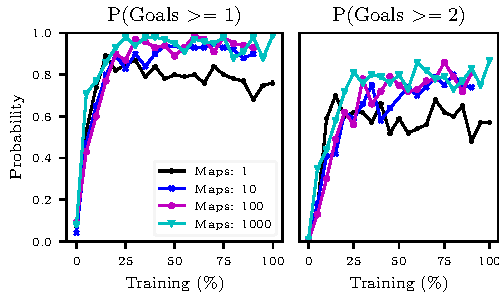
\includegraphics[width=\columnwidth]{images/plot_probability_3D-1000.pdf}
\caption{Probability of hitting a number of goals}
\label{fig:plot_reward_on_testing}
\end{figure}

\begin{figure}
\end{figure}

\begin{figure*}[h]
\centering     
\def\figwidth{\columnwidth}
\subfigure[Gridworld-Training]{\label{fig:a1}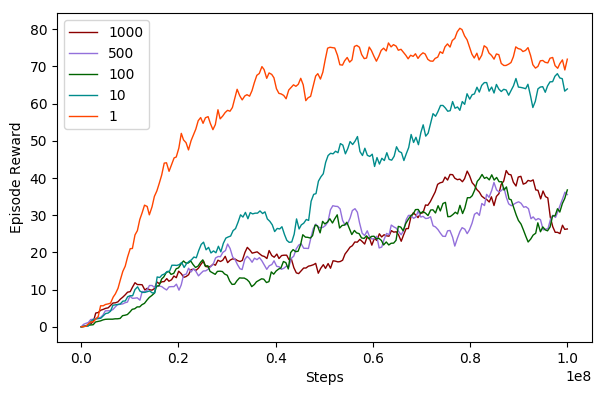
\includegraphics[width=\columnwidth]{gridworld-training.png}}
\subfigure[Gridworld-Testing]{\label{fig:b1}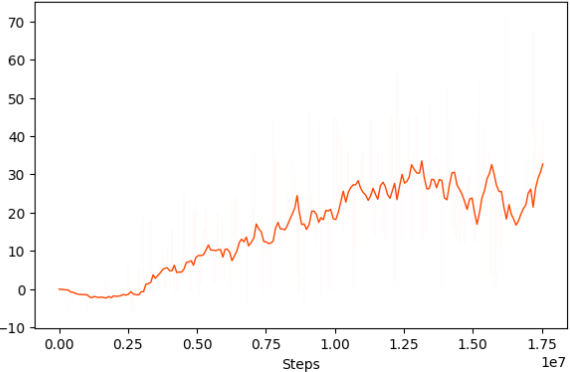
\includegraphics[width=\columnwidth]{plot-example.png}}
\subfigure[2DWorld-Training]{\label{fig:a2}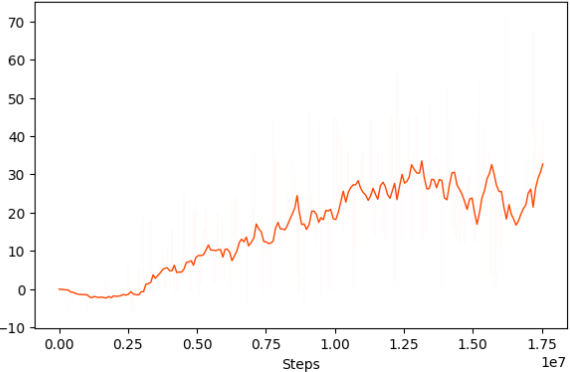
\includegraphics[width=\columnwidth]{plot-example.png}}
\subfigure[2DWord-Testing]{\label{fig:b2}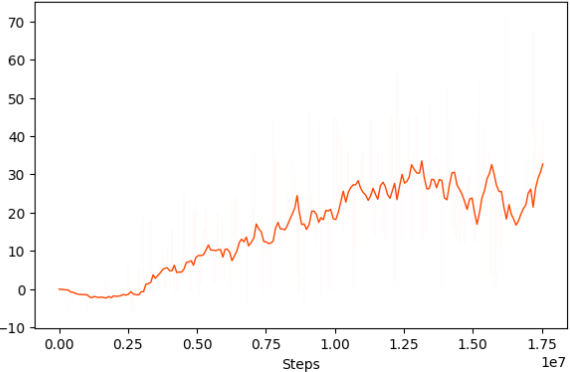
\includegraphics[width=\columnwidth]{plot-example.png}}
\subfigure[Lab-Training]{\label{fig:a3}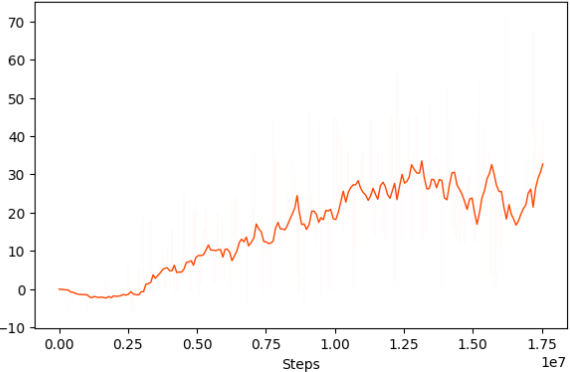
\includegraphics[width=\columnwidth]{plot-example.png}}
\subfigure[Lab-Testing]{\label{fig:b3}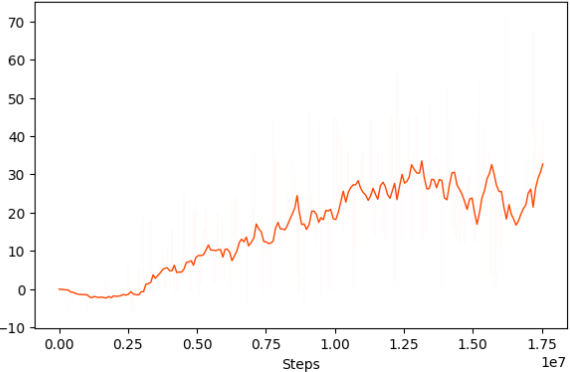
\includegraphics[width=\columnwidth]{plot-example.png}}
\label{fig:training-plots}
\end{figure*}

{\fontsize{9.0pt}{10.0pt} \selectfont
\bibliography{/z/home/dhiman/wrk/group-bib/shared}
%\bibliography{shared}
\bibliographystyle{aaai}
}
\end{document}
